\begin{abstract}
	数值方法作为解决科学和工程问题的一个强有力工具,它在许多基础研究和工程应用上扮演着重要的角色。
	随着数学理论和计算机硬件的发展,各种数值方法的提出,新的数值方法或其新的应用使相关领域取得了重要进展。
	本文主要聚焦于数值方法在机器学习领域,尤其是在深度学习领域中的应用。
	机器学习算法常常需要用到大量的数值计算,因为计算复杂度,我们往往无法直接得出精确的符号解。
	同时,由于计算过程中存在的种种误差,不考虑误差得到的计算结果往往与正确的结果大相径庭。
	为了解决这些问题,数值方法的提出为我们带来了可靠的理论分析工具,以及将计算不可行问题转化为计算可行的精确近似解问题的一系列工具。
	数值方法在机器学习领域的应用包括但不限于:
	\begin{enumerate}
		\item 数值稳定性问题
%		\item 迭代法求精确近似解
		\item 矩阵的特征分解及其应用
	\end{enumerate}
	本文主要将围绕上述两个个主题总结和讨论数字方法在机器学习领域的应用。

	% 关键词用“英文逗号”分隔
	\thusetup{
		keywords = {数值方法, 机器学习},
	}
\end{abstract}

\chapter{概述}
\label{chap:intro}
数值方法是数学的一个分支,它涉及解决科学应用中出现的概率问题的数值算法的理论基础。
这门学科涉及到各种问题,从函数和积分的近似到代数方程、超越方程、微分方程和积分方程的近似解,特别强调数值算法的稳定性、准确性、效率和可靠性。
数值方法是一门贴近实际生活问题的一门课程,它试图以最有效,最现实的方式解决各种数学和工程问题。
从维基百科的介绍中\footnote{\url{https://en.wikipedia.org/wiki/List_of_numerical_analysis_topics}},我们可以看到数值方法几乎无处不在。
本文重点介绍数值方法在机器学习方向中的应用,在第~\ref{chap:num_cond}章中我们主要介绍在机器学习算法中,数值稳定性带来的计算问题,包括数值溢出以及病态条件。
%因为机器学习的算法中往往存在大量的无法直接计算出符号解的问题,在第~\ref{chap:iter}章中我们将介绍如何使用迭代法将计算不可行的问题转化为计算可行的精确近似解求解问题。
接着,我们在第~\ref{chap:matrix_decom}章详细介绍矩阵特征值分解及在机器学习领域中的应用。
最后,第~\ref{chap:conclusion}章总结了数值方法中这三类问题在机器学习领域中的应用。

\chapter{数值稳定性问题}
\label{chap:num_cond}
一个数学问题在进行数值计算时,常常会遇到各种各样的数值问题。
这些数值问题主要有:
\begin{enumerate}
	\item 来输入数据的误差
	\item 舍入误差
	\item 截断误差
	\item 计算过程中的误差
\end{enumerate}

由于计算机只能用有限精度来表示浮点数,这会造成数值存储和计算过程中存在大量的舍入误差和截断误差。
甚至在数字计算机上计算一个数学函数,当函数涉及实数时,因为不能用有限的内存来精确表示,该计算就会变得很困难。

\section{数值上溢和下溢}
因为计算机只能表示有限精度的数字并且采用二进制表示数字而不是十进制,而实数域上数学运算经常涉及到无穷位数的无理数。
也就是说,对于几乎所有实数,我们在使用计算机处理这些数字的时候都可能遇到舍入误差或者截断误差。
所以实数域上的连续数学的求解就成了一个最基础的困难点。
虽然对于某个特定的实数,它的舍入误差(或截断误差,以下统一叫做截断误差)带来的相对误差可能很小,但是对于一个算法,尤其是涉及到很多运算操作的时候。
如果误差不能在运算过程中被减小,累积下来的误差将会变得非常大!
这样就会导致算法出错。
截断误差带来的一种毁灭性问题就是\textbf{数值下溢(uderflow)},具体来说,就是当一个很接近 $0$ 的数被截断为 $0$ 时带来的问题。
比如说,对于分数的分母 $\frac{1}{x}$ 以及 $log(x)$ 函数,如果参数为 $0$,它的结果是 $\infty$,这在很多的计算机软件中会导致异常报错或者在后续计算中得到一个非数字(not-a-number)的结果。
对于很多函数,参数为一个很接近 $0$ 的数或者直接为 $0$ 时有着天壤之别。
另一个由截断错误带来的很危险的数值问题就是\textbf{数值上溢(overflow)}。
具体来说,一个很大的数 $N < \infty$ 会因为计算机的有限精度被舍入到 $\infty$,这就会导致后续的计算出问题。

在机器学习中一个需要细心考虑数值问题的例子就是\textbf{softmax 函数}。
softmax 函数用于将任意的向量归一化为概率分布,也就是说输入向量各个元素的和将会归一化为 $1$。
它被定义为:
\begin{equation}
	\text{softmax}(\boldsymbol{x})_i = \frac{\exp(x_i)}{\sum_{j=1}^n\exp(x_j)}
\end{equation}
其中 $\boldsymbol{x}$ 是一个长度为 $n$ 的向量。

如果 $\boldsymbol{x}$ 中的每一元素都是一样的实数 $c$,我们可以很容易得出其 softmax 输出的每一个元素都是一样的,并且都为 $\frac{1}{n}$。
理想很美好,而如果不考虑数值问题,实际在计算机运算过程中却常常遇到各种麻烦。
例如当 $-\infty < c \ll 0$ 时,也就是说 $c$ 是一个远小于 $0$ 当不等于 $-\infty$ 的大数时。
假设 $c$ 本身没有出现数值问题,但是 $\exp(c)$ 依然会因为 $c$ 过小而使得其计算结果数值下溢为 $0$,这样会导致 softmax 输出为 $\frac{0}{0}$ 的形式,这样的结果时未定义的,总之我们无法得出正确的结果 $\frac{1}{n}$。
同样的,当 $0 \ll c < \infty$ 时,$\exp(c)$ 会因为指数爆炸的问题,非常容易上溢为 $\infty$。
这样就会导致 softmax 的输出为 $\frac{\infty}{\infty}$ 的形式,这同样是未定义的。
为了解决 softmax 带来的数值问题,我们可以令 $\boldsymbol{x}^* = \boldsymbol{x} - \max_i x_i$。
并且我们可以通过简单的推导验证上面的小 trick 不会影响最终的计算结果,但是同时能够轻松地避免数值问题\footnote{当然,当 $x$ 中不同元素之间的差距过大时,该 trick 很有可能还是无法避免数值问题的发生。}。

因此,当我们要用代码实现这些基础运算时,我们一定要特别注意这些数值问题的发生。
不过在日常开发中,我们往往会直接使用已有的深度学习函数库(例如,Theano~\cite{theano} 和 PyTorch~\cite{pytorch})来完成这些操作,而这些函数库的实现一般都会考虑好这些数值问题并且在出现数值问题时进行自动检测。
所以,在我们实现深度神经网络时,对于基础运算,如果深度学习函数库中已有实现,我们应当其自带的操作,而不是自己实现一个新的。
因为自己实现的时候往往容易忽略很多类似数值问题这样的工程问题。

\section{病态条件}
\textbf{条件(conditioning)}指输入的细微变换会对某个操作(函数)的结果带来多大的变化。
如果输入的细微变化导致操作的输出产生巨大的变化时,我们就认为该操作是\textbf{病态(ill conditioning)}的。
就像上节所描述的,计算机用有限精度表示实数时带来的舍入误差或截断误差就是输入的细微变化。

例如,对 $f(\bm{x}) = \bm{A}^{-1} \bm{x}, \bm{A} \in \mathbb{R}^{n \times n}$,如果 $\bm{A}$ 可以被特征分解为 $\lambda_1, \cdots, \lambda_{\text{rank } \bm{A}}$。
则它的条件数就是:
\begin{equation}
	\left|\frac{\max_{i} \lambda_i}{\min_j \lambda_j}\right|
\end{equation}

当条件数为大,上述运算 $f(\bm{x})$ 的结果对输入误差就越敏感。
病态矩阵会对之前运算产生的误差起到放大作用,在深度神经网络中,存在大量的矩阵乘法运算,所以我们应该尽量避免病态矩阵。

%\chapter{迭代法求精确近似解}
%\label{chap:iter}
%通过迭代来不断更新对某个数学问题的近视解,而不是直接得出一个可以求出符号解的公式。

\chapter{矩阵特征分解}
\label{chap:matrix_decom}
在机器学习和统计学中,我们经常要处理结构性数据,这些结构性数据一般用行和列的表格,或者矩阵来表示。
机器学习中的很多问题都可以使用矩阵代数和向量微积分来解决。
在这章中,我们将讨论一些可以使用矩阵分解技术解决的问题。
同时,还将讨论哪些特定的分解技术已经被证明对一些机器学习问题比较有效。

对于矩阵 $\bm{A} \in \mathbb{R}^{n \times n}$, 若 $\exists \lambda \in \mathbb{R}, x \in \mathbb{R}^n$,使得:
\begin{equation}
	\bm{Ax} = \lambda \bm{x}
\end{equation}

则称 $\lambda, \bm{x}$ 为 $\bm{A}$ 的特征值及其特征向量。
并且一个矩阵可以有多组特征值和特征向量。
在《数值方法》的第五章节中我们将会学习使用幂迭代法和 QR 法求解矩阵的特征分解。
本文的重点不在于介绍这些特征分解的计算方法,而是在于介绍其在机器学习领域的应用。
后续的小节中将依次介绍矩阵的特征分解的各种应用。

\section{主成分分析}
\textbf{主成分分析(Principal Components Analysis, PCA)}~\cite{PCA}是一种有损压缩算法,也就是说我们可以使用使用更少信息的主成分来尽可能少损失信息地恢复成原矩阵。
形式化地描述为,对于数据矩阵 $\bm{X} \in \mathbb{R}^{n \times p}$,我们希望用一个更低维度的压缩版本 $\tilde{\bm{X}} = \bm{X}\bm{D}^\top\in \mathbb{R}^{n \times q}, q \ll p$ 来描述 $\bm{X}$。
使得我们可以通过简单运算 $\bm{X} \approx \tilde{\bm{X}} \bm{D}$ 来将压缩版本恢复到原矩阵,其中通过推导可以得到 $\bm{D} \in \mathbb{R}^{q \times p}$就是 $\bm{X}^\top \bm{X}$ 最大的 $q$ 个特征值对应的特征向量组成的矩阵。
不过上述 $\bm{X}^\top \bm{X}$ 的特征分解计算量很大,还可以继续使用奇异值分解(SVD)对其进一步优化。

PCA 的应用有:

\begin{enumerate}
	\item 神经科学中的尖峰触发协方差分析
	\item 量化金融
	\item 图像压缩
	\item 面部识别
	\item 医疗数据关联
\end{enumerate}

\section{低秩估计}
通过 Eckart-Young 定理~\cite{Eckart1936_lowrank}:
\begin{equation}
	\min_{\text{rank}(\bm{Y}) = r} \lVert \bm{X} - \bm{Y} \rVert_F^2
\end{equation}
的解为 $\bm{Y} = \sum_{i=1}^r \sigma_i \bm{u}_i \bm{v}_i^\top$ 其中 $(\sigma_i, \bm{u}_i, \bm{v}_i)$ 来自 $\bm{X}$ 的 SVD 分解 $\bm{U\Sigma}\bm{V}^\top$。

\begin{figure}
	\begin{minipage}{.5\linewidth}
		\centering
		\subfloat[原图]{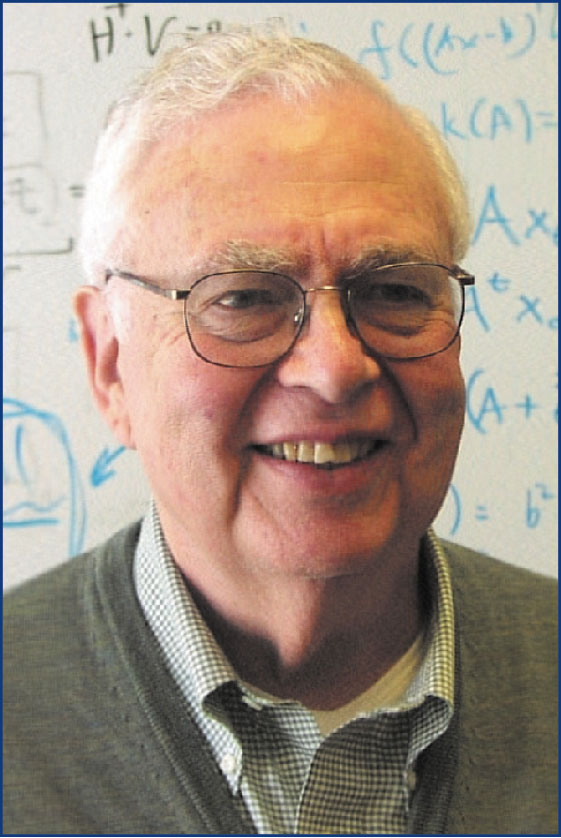
\includegraphics[width=.475\columnwidth]{raw_pic.jpg}}
	\end{minipage}%
	\begin{minipage}{.5\linewidth}
		\centering
		\subfloat[rank 120]{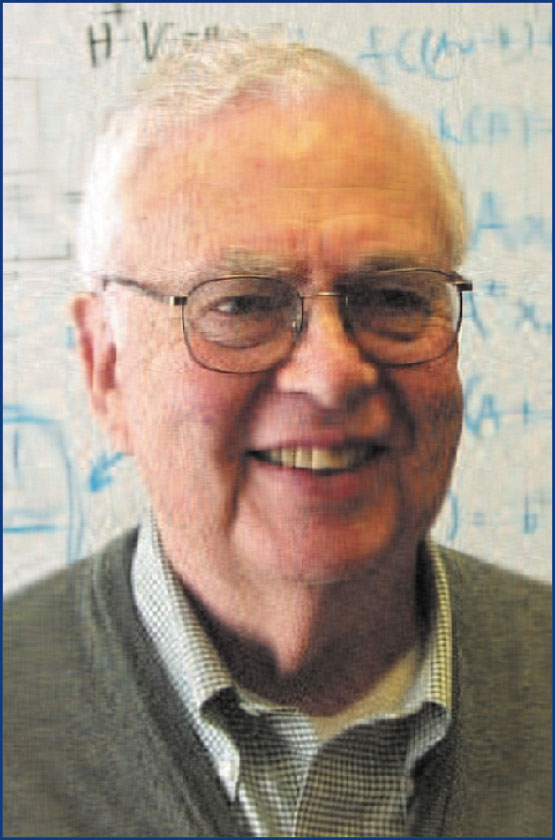
\includegraphics[width=.475\columnwidth]{rank_120.jpg}}
	\end{minipage}\par\medskip
	\centering
	\subfloat[rank 50]{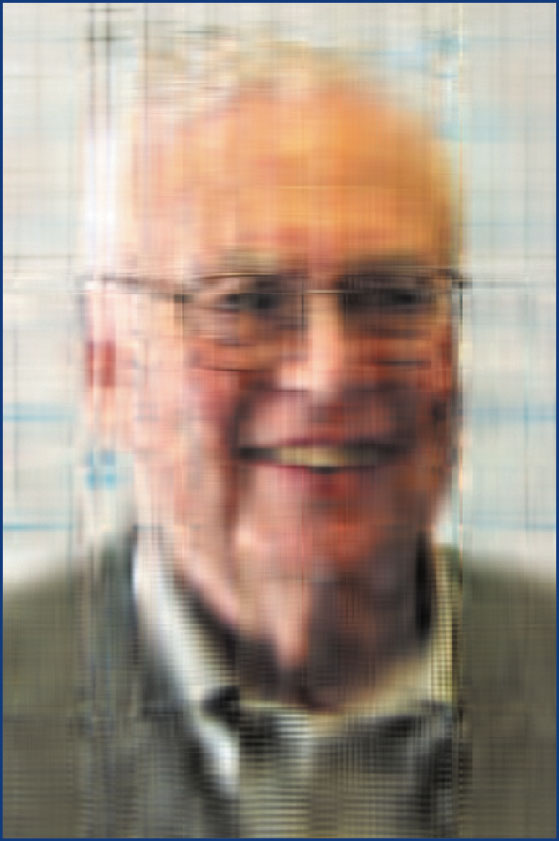
\includegraphics[width=.2375\columnwidth]{rank_50.jpg}}
	\caption{低秩估计用于图片压缩}
	\label{fig:low_rank}
\end{figure}

虽然低秩估计的形式非常类似于 PCA,不过他们的公式是不一样的。
低秩估计的应用方向也有点类似 PCA,主要包括图像和数据的压缩。
图~\ref{fig:low_rank}展示了低秩估计用于图片压缩的一个例子。
原图是一个 $897 \times 598$ 大小的图片,如果不采用任何压缩的话需要 $897 \times 598 \times 3 \times 8 = 12,873,744$ 字节。
如果我们采用 rank 120 估计,则需要 $120 \times (897 \times 3 + 598) \times 8 = 3,157,440$ 字节,同理 rank 50 和 rank 12 分别需要 $1,315,600$ 和 $315,744$ 字节。
我们可以看出,压缩比例还是挺高的,并且从图中可以看出来在压缩比例 $25\%$ 时图像依然挺清晰的。

\section{线性回归}
线性回归作为一种最简单的机器学习算法,对于线性回归,对于 SVD 分解 $\bm{X} = \bm{U\Sigma}\bm{V}^\top$,我们有:
\begin{align}
	\begin{split}
		\hat{\beta} &= (\bm{X}^\top\bm{X})^-\bm{X}^\top\bm{y} \\
		&= (\bm{V\Sigma}^2\bm{V}^\top)^+\bm{V\Sigma U}^\top\bm{y} \\
		&= \sum_{i=1}^r \left(\frac{\bm{u}_i^\top \bm{y}}{\sigma_i}\right)\bm{v}_i
	\end{split}
\end{align}

一般来说,SVD 比其他矩阵分解方法(例如 QR)需要更多的计算量。
但是在某些应用中,SVD 是为了其他目的而计算出来的话,然后我们可以用 SVD 的结果高效地得到最小二乘法。

\begin{figure}[H]
	\centering
	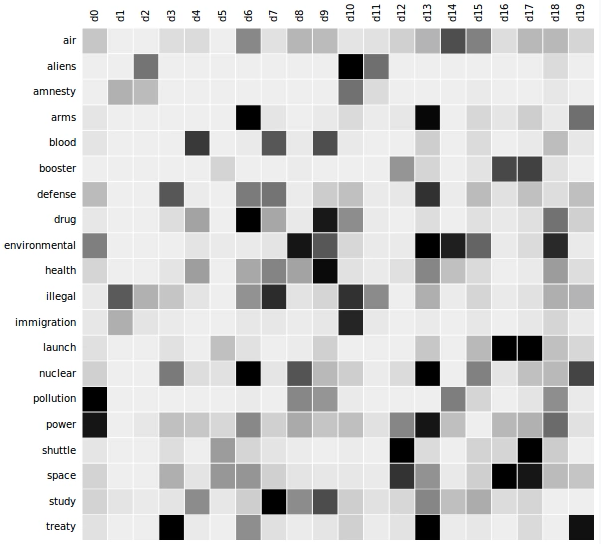
\includegraphics[width=14cm]{topic_model.png}
	\caption{文档-词矩阵}
	\label{fig:topic_model}
\end{figure}

\section{主题模型}
在机器学习和自然语言处理中,\textbf{主题模型(topic modeling)}~\cite{topic_model}是一种用于发现文档集合中出现的抽象 “主题” 的统计模型。
在文本挖掘工具中,主题模型经常被用于发现文本正文中隐藏的语义结构。

一个主题可以是任何东西,从一个歌曲流派到一个动物种类。
给定一个文档是关于一个特定的主题,我们就会期望特定的词在文档中出现的频率会更高或更低。
“狗”和 “骨头”在关于狗的文件中出现的频率较高,“猫”和 “喵”在关于猫的文件中出现的频率较高,而 “他”和 “她”在两者中出现的频率相同。
一篇文档通常以不同的比例处理多个主题,因此,在一篇10\%关于猫和90\%关于狗的文档中,狗的词可能会比猫的词多9倍左右。

做主题建模的一种方法是用文档-词矩阵的形式来表示文本数据的语料库,如图~\ref{fig:topic_model}所示。
每一列对应一个文档,每一行对应一个单词。
一个单元格存储了一个词在文档中的频率——深色单元格表示词的频率高。
由此产生的模式被称为 “主题”。
我们可以采用多种方式来构建主题模型,这里以 SVD 为例。

使用矩阵分解进行主题建模的一般思路是:
考虑最极端的情况——用两个向量的外积重建矩阵。
显然,在大多数情况下,我们无法精确地重建矩阵。
但如果我们有一个向量是每个词汇在总字数中的相对频率,一个是每个文档的平均字数,那么这个外积将是我们能得到的最接近的。
我们在主题建模中的目标是将不同的主题从文本集合中分离出来。
我们期望在一个主题中出现频率较高的词在另一个主题中出现频率较低——否则这个词就不是分离出两个主题的好选择。
用线性代数术语来说,我们可以说,我们期望主题是正交的。
SVD 将一个矩阵分解为一个具有正交列的矩阵和一个具有正交行的矩阵,以及一个对角矩阵,其中包含每个分解因子的相对重要性。
对于主题建模,我们使用文档的词包(Bag-of-Words)表示,并将其分解为两个非负矩阵的乘积,SVD 中 $\Sigma$ 的阶数便是主题数量。

\begin{figure}[!htp]
	\centering
	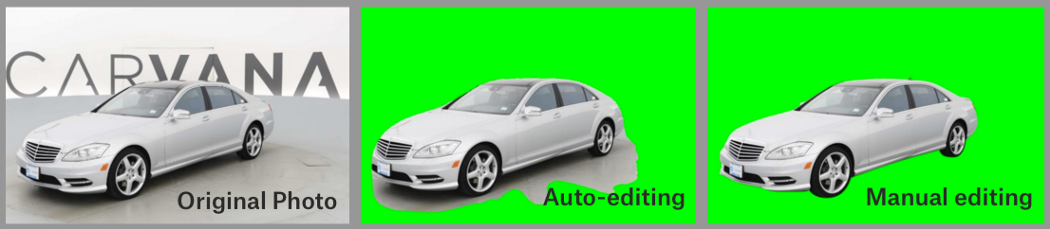
\includegraphics[width=0.9\columnwidth]{remove_car_bg.png}
	\caption{去除汽车照片的背景}
	\label{fig:rm_car_bg}
\end{figure}

\begin{figure}[!htp]
	\centering
	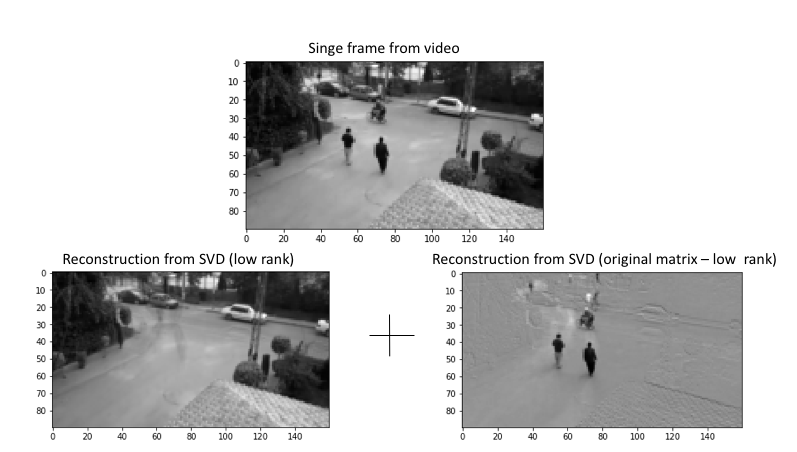
\includegraphics[width=0.9\columnwidth]{rm_bg.png}
	\caption{背景前景分离}
	\label{fig:rm_bg}
\end{figure}

\section{去除图像背景}
自动去除背景有很多用例,例如,Kaggle 的 Carvana 图像遮挡挑战赛,开发了一种自动去除照片背景的算法。
对于大多数电商网站来说,要想提高销售量,照片背景去除服务是不可或缺的。
去除照片背景可以突出产品,比如图~\ref{fig:rm_car_bg}中所展示的。

在视频中把前景和背景分开,也让我们可以选择用背景做一些有趣的事情。
像 Snapchat 这样的移动应用有可能将其作为一项附加功能。
最先进的背景去除方法使用神经网进行图像分割,但为此我们需要标记数据来训练神经网。
这就是矩阵分解可以用于背景去除的地方,因为它为未标记的视频数据提供了一个良好的基线方法。

奇异值分解提供了一种从视频中分离背景和前景的巧妙方法。
其思路是将视频分割成帧(就是一组图像),将每幅图像做成一个一维向量,并将这些一维向量与每幅图像对应的一维向量水平堆叠成一个矩阵。
在该矩阵中,大部分的行向量看起来几乎是一样的,代表了图像中在所有帧中不变的部分(背景),但是有一些区域的晃动图案看起来不同。
这个想法是,整体看起来相似的图案是背景,而晃动的部分是在不同帧中不恒定的东西——比如一个行走的行人或一辆移动的汽车。
所以我们可以使用 SVD 来分离前景或背景,我们可以用特征值最小对应的向量重构出背景,然后我们将原图减去背景就可以得到前景。
图~\ref{fig:rm_bg}展示了利用 SVD 进行背景前景分离的过程。

\chapter{结论}
\label{chap:conclusion}

本文从数值问题和矩阵的特征分解两个方向展开,介绍了数值方法在机器学习领域的应用。
学习了数值方法后,我们面对机器学习的算法时,我们不仅要掌握理论的推导,更加要时刻注意这些大量的计算中可能出现的各种数值问题,譬如数值溢出或者病态条件。
这样我们便可以基于数值方法的分析结果,合理修改公式,避免出现数值问题。
相比数值问题这种在底层运算上出现的问题,数值方法也广泛应用于矩阵的特征值分解中。
数值方法不仅要求足够准确地求出矩阵地求出特征值分解,更要注重算法的复杂度,以求快速高效地求解。
利用特征值分解,我们可以用主成分分析和低秩估计来做数据压缩以及降噪。
我们还能对文本进行主题模型来将文档进行分类,也可以对图像分离其背景和前景。
更多的应用还包括使用迭代法求解深度学习中的优化问题~\cite{adam},使用泰勒估计使用梯度信息来对抗模型~\cite{adversarial}。